% \input{\pSections "sec-plots"}


% worst-sequence-04.nb
% /Users/dantopa/primary-repos/github/experiment-mathematica/nb/rcs/fourier/worst/
% user: dantopa, CPU: Xiuhcoatl, MM v. 12.0.0 for Mac OS X x86
% 13:09:20 Apr 30, 2020

%     %     %     %     %     %     %     %     %
\subsection{Models of Increasing Fidelity}

%
\begin{table}
    \begin{center}
        \begin{tabular}{cccc}
                %
            $d$ & Data and Fourier Representation & Residual Fit Error & Total Error for Fit Sequence \\\hline
                %
                %
            \raisebox{2.25cm}{$d=2$}
                & \includegraphics[ scale=  0.35 ]{\pLocalGraphics nu=16-d=02-A}
                & \includegraphics[ scale=  0.35 ]{\pLocalGraphics nu=16-d=02-B}
                & \includegraphics[ scale=  0.35 ]{\pLocalGraphics nu=16-d=02-C} \\[5pt]
                %
                %
            \raisebox{2.25cm}{$d=20$}
                & 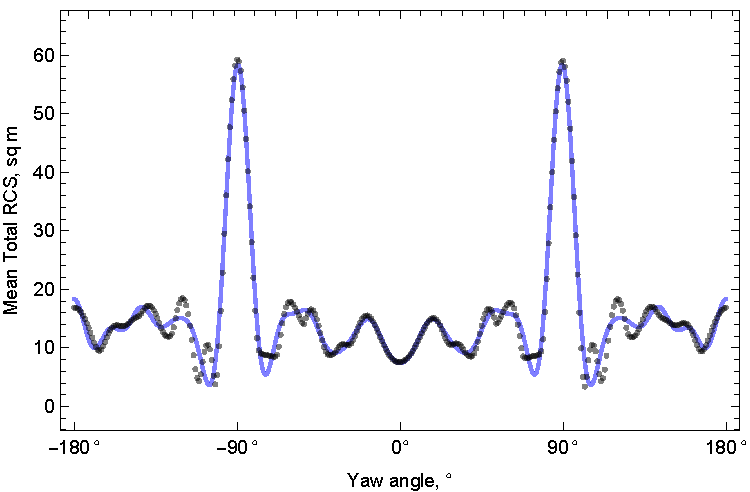
\includegraphics[ scale=  0.35 ]{\pLocalGraphics/nu=16-d=20-A}
                & 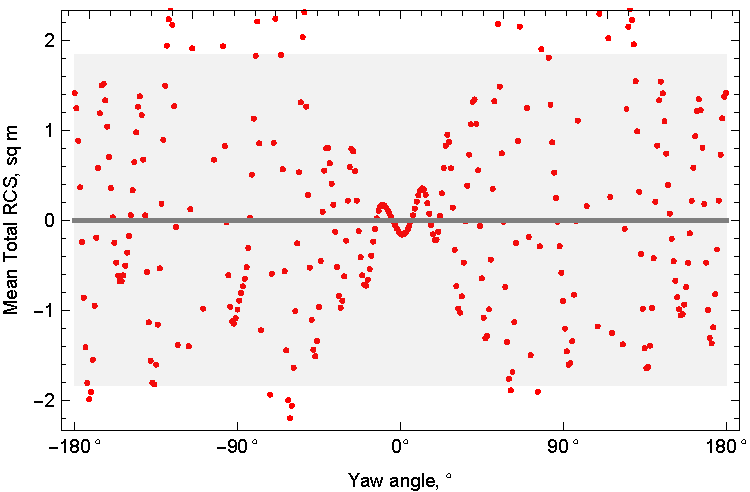
\includegraphics[ scale=  0.35 ]{\pLocalGraphics/nu=16-d=20-B}
                & 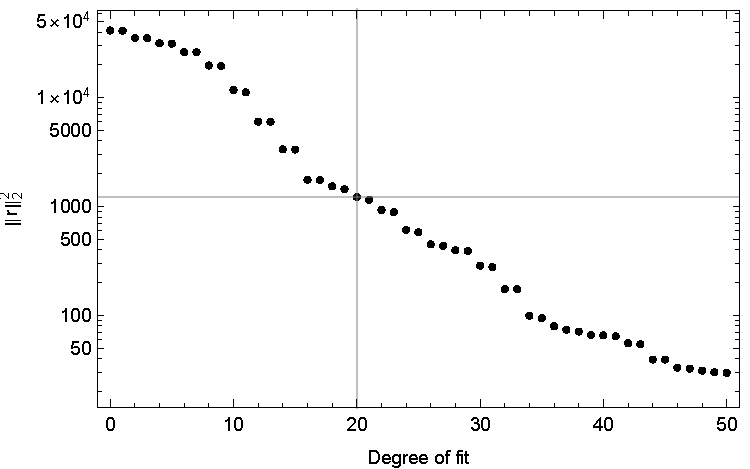
\includegraphics[ scale=  0.35 ]{\pLocalGraphics/nu=16-d=20-C} \\[5pt]
                %
                %
            \raisebox{2.25cm}{$d=40$}
                & 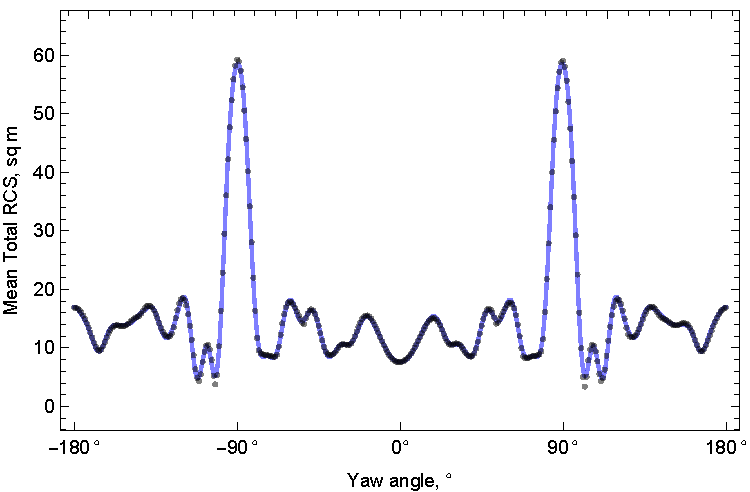
\includegraphics[ scale=  0.35 ]{\pLocalGraphics/nu=16-d=40-A}
                & 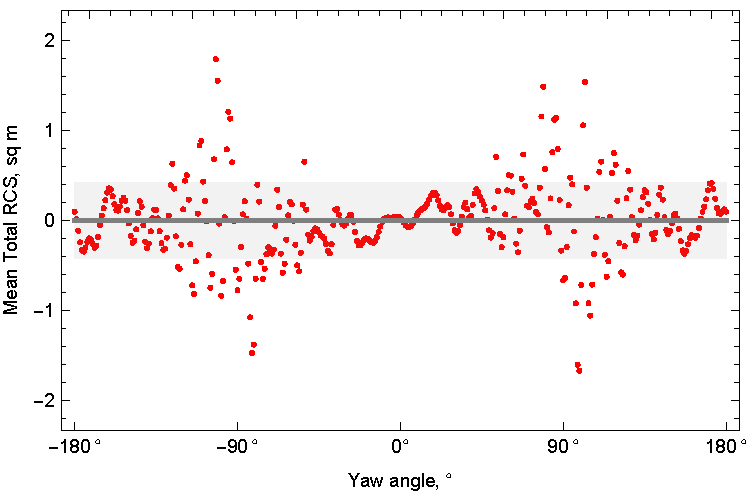
\includegraphics[ scale=  0.35 ]{\pLocalGraphics/nu=16-d=40-B}
                & 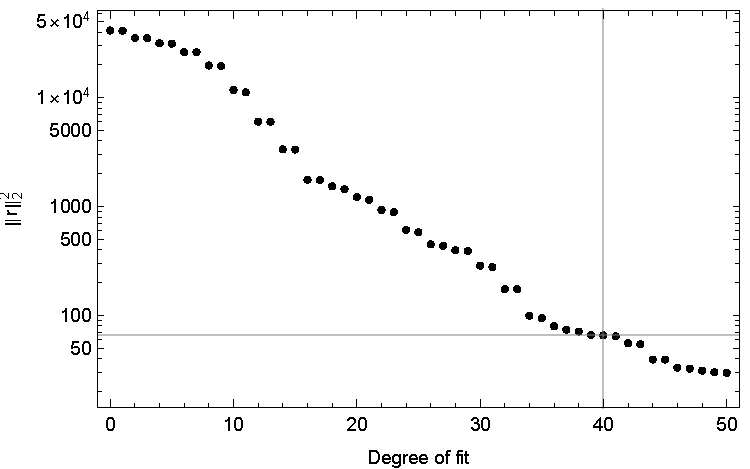
\includegraphics[ scale=  0.35 ]{\pLocalGraphics/nu=16-d=40-C} \\[5pt]
                %
                %
		%
        \end{tabular}
    \end{center}
\label{tab:panels}
\end{table}

\begin{table}
    \begin{center}
	\caption{Seeing the uncertainties in the fit parameters.}
        \begin{tabular}{cccc}
                %
           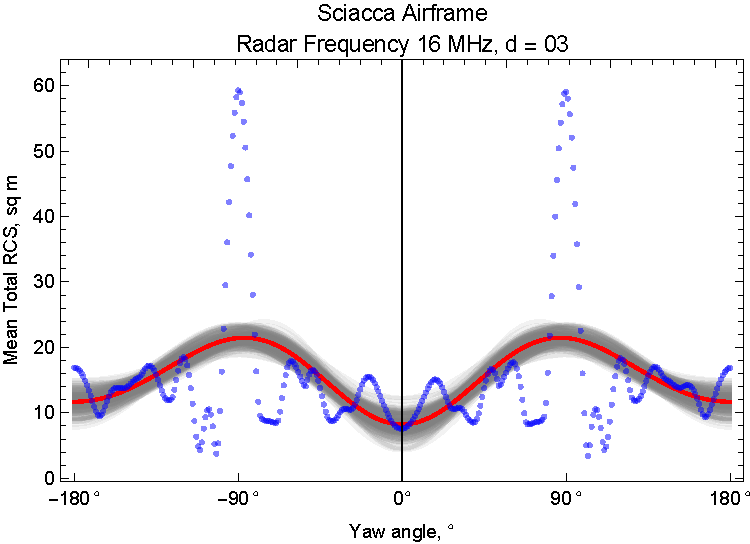
\includegraphics[ scale =  0.35 ]{\pLocalGraphics fits/wh-fourier-16Mhz-d03} &
           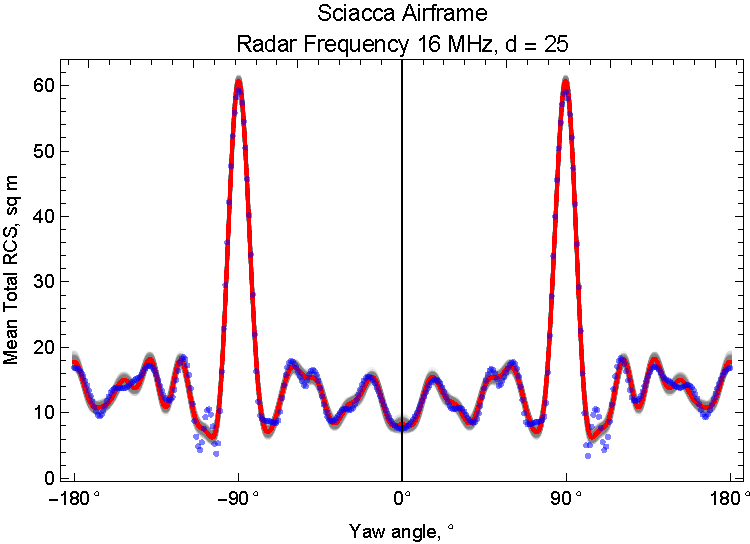
\includegraphics[ scale =  0.35 ]{\pLocalGraphics fits/wh-fourier-16Mhz-d25}
		%
        \end{tabular}
    \end{center}
\label{tab:straws}
\end{table}

\endinput  %  ==  ==  ==  ==  ==  ==  ==  ==  ==
